\documentclass[a4paper,10pt]{article}

\usepackage[utf8]{inputenc}
\usepackage[hungarian]{babel}
\usepackage{t1enc}
\usepackage{listings}
\usepackage{textcomp}
\usepackage{graphicx}
\usepackage{float}
\usepackage{url}

%opening
\title{Hello Window! - GTK+/gtkmm programozás GNU/Linux alatt}
\author{Pfeiffer Szilárd}
\date{\today}

\begin{document}

\pagenumbering{roman}

\begin{titlepage}

\maketitle

\begin{abstract}
A \textit{GTK+} (\textit{GIMP Toolkit}) egy \textit{C} nyelven -- ám objektum-orientált megközelítéssel -- íródott, grafikus felhasználói felületek (\textit{GUI}) létrehozására használatos alkalmazás-programozási interfész. A \textit{gtkmm} nem más, mint ennek a függvénykönyvtárnak a \textit{C++} változata, pontosabban fogalmazva \textit{wrapper}e. Mindkét terjesztése \textit{LGPL} licenc alatt történik, így bátran felhasználható mind szabad/ingyenes, mind kereskedelmi szoftverek létrehozására.

A most kezdődő sorozat célja az abszolút kezdetektől indulva bemutatni a \textit{GTK+} és a \textit{gtkmm} hasonlóságait, különbözőségeit, sajátosságait eljutva egy olyan szintre, ahol remélhetőleg a több éves tapasztalattal rendelkező fejlesztők is találnak hasznos, megfontolásra érdemes ötleteket, információkat.
\end{abstract}

\pagebreak

\tableofcontents

\end{titlepage}

\pagenumbering{arabic}

\section{Bevezetés}

Már a legegyszerűbb felhasználói felület láttán is könnyen belátható, hogy a korábbi példaprogramjaink kissé sántítanak, mégpedig abban a tekintetben, hogy nincs olyan valós életben is használt program amiben egy-egy \textit{widget} lenne csupán. Ha viszont több \textit{widget}et szeretnénk elhelyezni egy ablakban kézenfekvő kérdés, hogy miként tudnák őket a felületen csoportokba rendezni. Erre a kérdésre keressük a választ ebben a részben.

\section{Fogalmak}

A korábbiakhoz hasonlóan itt is érdemes először tisztázni néhány alapfogalmat és csak utána kezdeni bele az érdemi munkába.

\subsection{Konténerek}
\index{konténer}

A \textit{widget}ek a felületen történő csoportokba csoportokba rendezése konténerek (\textit{container}) segítségével valósul meg. Ezek olyan láthatatlan \textit{widget}ek, melyekbe más \textit{widget}eket helyezhetünk (\textit{pack}).

\index{\texttt{Gtk::Container}}
A \texttt{GtkContainer}, avagy \texttt{Gtk::Container} egy önmagában nem használható absztrakt osztály, mely csupán ősül szolgál minden olyan származtatott osztálynak, melyet widgetek tárolására lehet használni.

\index{\texttt{Gtk::Bin}}
\index{\texttt{Gtk::Box}}
Alapvetően két ilyen leszármazott osztálytípussal találkozhatunk a későbbiekben. Ezek a \textit{bin} és \textit{box} ősosztályok, melyek maguk is absztraktak és abban különböznek egymástól, hogy hány elem tárolására alkalmasak. Előbbiek összesen egyére, míg az utóbbiak akárhányéra.

\subsubsection{Egy elemű konténerek}

\label{sec:bin}
\index{\texttt{Gtk::Bin}}
A \texttt{GtkBin} jelentősége a további származtatásoknál jelentkezik majd, hisz az olyan nélkülözhetetlen típusoknak, mint az ablak (\texttt{GtkWindow}), a gomb (\texttt{GtkButton}), vagy a frame (\texttt{GtkFrame}) mind a \textit{GtkBin} az ősosztálya.

\subsubsection{Több elemű konténerek}

\index{\texttt{Gtk::Box}}
\index{\texttt{Gtk::HBox}}
\index{\texttt{Gtk::VBox}}
\index{\texttt{Gtk::Table}}
A felületi elrendezés kialakításakor játszik fontos szerepet, hisz a benne található \textit{widget}ek -- amit a \textit{GTK} konténer gyerekeinek (\textit{children}) nevez -- elrendezésén túl azok méretét és konténeren belüli pozícióját is meghatározza. Ilyen típusok például a horizontális, vagy vertikális rendezést biztosító boxok (\texttt{GtkHBox}, \texttt{GtkVBox}), vagy a táblázatos megjelenítést szolgáló \texttt{GtkTable}.

\subsection{Méretezés}

\index{\textit{size request}}
\label{par:widgetsizerequest}
A \texttt{GtkContainer} osztály legfontosabb funkcionalitása -- melyet minden származtatott osztály is felhasznál -- az, hogy meg tudja határozni a benne található elemek méretét. Ezt persze nem teljesen önállóan teszi, hanem megkérdezni a benne található \textit{widget}eket, hogy mekkora helyre lenne szükségük. Minden egyes \textit{widget} saját hatáskörben állapíthatja meg, hogy mekkora az a vízszintes, illetve függőleges kiterjedés, ami az igényeinek legjobban megfelelne. Ezt az méretigényt nevezi a \textit{GTK} \textit{size request}nek. Ez a mechanizmus fentről lefelé, azaz a gyökértől a levelek felé terjed abban a fa hierarchiában, melynek gyökere az ablak, közbülső elemeit a konténerek, leveleit pedig a widgetek alkotják.

\index{\textit{size allocation}}
\label{par:widgetsizeallocation}
A legegyszerűbb és legáltalánosabb eset tehát az, hogy a konténerek -- amilyen maga az balak is -- összeadják a gyermekeik (a fában közvetlenül alattuk lévő elemek) méretigényét és azt sajátjukként propagálják. A valóság azonban nem ilyen demokratikus. Minden konténernek lehetősége van arra, hogy a benne lévő elemek felé -- egy az eredeti igénytől esetlegesen eltérő -- méretet (\textit{size allocation}) adjon vissza mellyel gazdálkodniuk kell és amely rájuk nézve kötelező érvényű.

\subsection{Elrendezés}

Normális esetben egy ablak rendelkezésre bocsájtja azt a területet, melyet a benne lévő \textit{widget}ek igényeltek. A kérdés nem is abban  áll, hogy mi legyen akkor ha pont annyi hely van amennyi kell, hanem sokkal inkább abban, miként jelenítse meg a konténer a saját \textit{widget}jeit, ha több a hely, mint amennyire feltétlenül szükség volna. Ilyen eset például akkor állhat elő, ha ez ablak átméretezhető és azt a felhasználó nagyobbra nyújtja, mint amekkora hely a benne lévő widgetek kirajzolásához minimálisan elégséges.

\index{\textit{fill}}
\index{\textit{expand}}
\index{\textit{pack-type}}
Ezt az esetet szabályozzák azok a paraméterek (pl: \textit{fill}, \textit{expand}, \textit{pack-type}, melyek tulajdonképpen sem a konténerhez, sem pedig a benne tárolt \textit{widget}hez nem tartoznak, hisz a kettejük viszonyát határozzák meg. Megadásuk akkor történik, amikor egy \textit{widget}et szeretnénk egy konténerben -- például egy \textit{box}ban -- elhelyezni.

A konténereket és ezen belül a \textit{box}okat leginkább úgy képzelhetjük el, mint egy dobozt -- vagy ha programozási szakszóval akarunk élni vermet -- melynek mindkét végére lehet pakolni. A verem hasonlat már csak azért is helytálló, mert az egyes elemek verembe történő elhelyezése csak egymást követően, csak egymásra lehetséges. Annyiban viszont sántít a példa, hogy a \textit{GTK} esetén rendkívül ritka -- bár egyáltalában nem lehetetlen -- hogy elemeket vegyünk ki egy konténerből.

\section{Alapműveletek}

Nyilvánvaló igény, hogy ha már vannak tárolóink és azokhoz kapcsolódóan \textit{widget}eink, akkor azokkal műveleteket lehessen végezni. Az sem túl meglepő, hogy ezt a különböző típusú konténerek esetén másként kell megtenni. Itt csak a legalapvetőbb műveleteket és típusokat vesszük sorra, azokat is csak abban a mértékben mely a koncepció megértéséhez szükséges.

\subsection{Létrehozás}

A \textit{GtkContainer}, \textit{GtkBin}, illetve a \textit{GtkBox} absztrakt osztályok, így ebben a formájukban nem, csak a származtatott osztályok révén példányosíthatóak. Ezek közül ebben a részben a vízszintes, illetve függőleges elrendezésű \textit{box}okat (\textit{GtkHBox}, \textit{GtkVBox}), illetve a táblázatot (\textit{GtkTable}) tárgyaljuk.

\subsubsection{\textit{GtkVBox} és \textit{GtkHBox}}

\index{\textit{homogeneous}}
\index{\textit{spacing}}
Függetlenül az iránytól a létrehozáskor két paramétert kell megadunk (\textit{homogeneous}, \textit{spacing}), ahol az egyik egyik egy \textit{bool}, melynek \textit{true} értéke esetén minden egyes elem azonos helyet foglal majd el a konténerben, míg a másik az egyes elemek között üresen hagyandó részt adja meg pixelben.

\subsubsection{\textit{Table}}

Létrehozáskor a táblázat sorainak, illetve oszlopainak kezdeti száma, valamint a korábbról ismert \textit{homogeneous} érték adandó meg. Míg a vízszintes elrendezésű \textit{box}oknál a \textit{widget}ek szélessége, a függőlegeseknél a magassága, addig a táblázatoknál mindkettő azonos ha a \textit{homogeneous} paraméter értéke \textit{true}.

\subsection{Elem hozzáadása}

Ezen függvények közös sajátossága, hogy paraméterként átveszik azt a \textit{widget}et, melyet a konténerbe kívánunk helyezni. A korábban említett fa hierarchiából következik, hogy egy elem nem lehet több szülőnek gyermeke (különben erdő szerkezetről beszélnénk), azaz egy \textit{widget}et összesen egy konténerben helyezhetünk el. Ha esetleg ezt másodszor is megpróbálnánk -- még mielőtt a korábbi konténeréből eltávolítottuk volna -- akkor futás idejű hibaüzenetet kapunk.

\index{referencia számlálás}
Ne feledjük, ahogy arról már említést tettünk, a \textit{GTK} rendelkezik referenciaszámlálási metódussal, azaz minden egyes objektum (\texttt{GtkObject}) -- esetünkben \texttt{GtkWidget} -- rendelkezik egy referenciaszámmal. Ha egy \textit{widget}et egy konténerbe helyezünk, annak referenciáját a konténer, annak rendje és módja szerint, növeli eggyel. Ez a referencia mindaddig megmarad, míg a \textit{widget}et el nem távolítjuk, vagy a konténer valamilyen oknál fogva meg nem szűnik, ami jellemzően akkor következik be ha az egész ablakot megszüntetjük (\textit{destroy}).

\subsubsection{\textit{Container}}

Az \texttt{add} nevű függvény egyetlen paramétert, az elhelyezni kívánt \textit{widget}et veszi át. Ritkán, leginkább csak egyszerű konténereknél alkalmazott hívás, lévén olyan alapértelmezett paraméterek használ a \textit{widget} elhelyezésére, melyek a felhasználó céljainak a legtöbb esetben nem felelnek meg.

Használható ugyan a származtatott, bonyolultabb konténerek esetén is (pl: \texttt{GtkBox}, \texttt{GtkTable}), de célszerűbb ilyen esetekben az azokhoz tartozó, specifikus függvényt alkalmazni, lévén az sokkal rugalmasabban paraméterezhetőek.

\subsubsection{\textit{Bin}}

Ebbe a típusba elemet csak a \texttt{GtkContainer} \texttt{add} függvényével tehetünk. Ha többször hívjuk meg a függvényt anélkül, hogy a \textit{GtkBin} gyerekét eltávolítanánk futási hibát kapunk, hiszen a \textit{GtkBin} csak egyetlen elem tárolására képes.

\subsubsection{\textit{Box}}

Ahogy arról a bevezetőben szó volt a \textit{GtkBox} típus olyan, mint egy két bemenetű verem. Ennek megfelelően két függvény van, amivel elemeket (egyet, vagy többet) lehet helyezni a konténerbe. A \texttt{pack\_start} függőleges elrendezés (\textit{GtkVBox}) esetén felülről lefelé haladva tölti meg a konténert úgy, hogy az egymást után elhelyezett elemek egymás alatt jelennek meg, míg a vízszintes elrendezést biztosító változat (\textit{GtkHBox}) balról jobbra haladva teszi ugyanezt. A \texttt{pack\_end} hívás ezekkel ellentétesen működik, tehát alulról, illetve jobbról balra haladva helyez elemeket a tárolóba.

\index{\textit{fill}}
\index{\textit{expand}}
\index{\textit{padding}}
Ahogy a \textit{GtkContainer} esetén, itt is megadandó a \textit{widget}, de ezen túl itt a konténeren belüli elhelyezkedést meghatározó értékek is paramméterek. Az \textit{expand} és \textit{fill} \textit{bool} típusú paraméterek, melyek a korábban már említett ''felesleges'' hely kitöltésére vonatkoznak. Előbbi azt határozza meg, hogy a \textit{widget} a konténeren belül rendelkezésre álló helyet kitöltse-e, azaz ha van ilyen akkor az igényelje-e magának (\textit{ture}), vagy lemondjon róla (\textit{false}) a többi -- a konténerben lévő -- \textit{widget} javára. Utóbbi paraméter annak beállítására szolgál, hogy a rendelkezésre álló -- illetve az \textit{expand} okán elnyert -- hellyel mi történjék. Ha a paraméter értéke \textit{true}, akkor a \textit{widget} maga tölti ki ezt a helyet, azaz a feltétlenül szükségesnél nagyobb helyen rajzolódik ki, míg ha az érték \textit{false}, akkor csak a minimálisan szükséges helyre rajzolódik és a maradék részt úgymond üresen hagyja. A \textit{pack} függvények utolsó paramétere a \textit{padding}, mely a \textit{widget} körül (\textit{GtkVBox} esetén felül és alul, \textit{GtkHBox} esetén jobbról és balról) hagyandó üres hely értékét adja meg pixelben.

Ha elsőre nem is teljesen világos, mit jelent ez a gyakorlatban, a következő fejezet illusztrációjából minden világossá válik.

\subsubsection{\textit{Table}}

Az \textit{attach} függvény -- mely a táblázatok esetén elem elhelyezésére szolgál -- kissé összetettebb, mint a korábbiak, lévén egy táblázatnál vízszintesen és függőlegesen egyaránt szükséges megadni a \textit{fill}, illetve \textit{expand} paramétereket, melyek kiegészülnek egy \textit{srink} opcióval is, ez azonban már túlmutat ennek a résznek a keretein.

\subsection{Elem eltávolítása}

A származtatott típusok, legalábbis azok, amelyekkel ebben a részben foglalkozunk (\textit{GtkTable}, \textit{GtkBin}, \textit{GtkBox}) nem igényelnek az eltávolítás során semmilyen extra műveletet, így a \textit{GtkContainer} funkcionalitására támaszkodnak.

\subsubsection{\textit{Container}}

\index{referencia számlálás}
A \texttt{remove} függvény értelemszerűen az eltávolítani kívánt \textit{widget}et várja paraméterként és ahogy azt említettük az általa tartott referenciát meg is szünteti. Ez jellemzően (a referenciaszámlálás \textit{GTK}-beli sajátosságairól egy késöbbi részben szólunk) azt is jeleni egyben, hogy az eltávolított \textit{widget}re az utolsó (hisz többnyire csak a konténere tart referenciát egy \textit{widgetre}) referencia és ezzel maga a \textit{widget} is megszűnik.

Ha ezt az esetet el akarjuk kerülni, akkor még az eltávolítás előtt a referenciaszám növeléséről magunknak kell gondoskodnunk. Vagyis, ha két lépésben (\texttt{remove} és \texttt{add}) akarunk egy \textit{widget}et áthelyezni egyik konténerből a másikba, akkor az eltávolítás előtt növelnünk, a hozzáadás után pedig csökkentenünk kell a referenciát. Utóbbira azért van szükség, mert az új szülőelem maga is növel egyet a referencián, így ha mi, a magunk által korábban megnövelt referenciát nem csökkentenénk, a widget soha nem szűnne meg.

Hasonlóan a \textit{GtkBin}hez itt sincs specifikus függvény az eltávolításra, hanem a \textit{GtkContainer} \texttt{remove} függvényét hívjuk.

\section{Pa(c)koljunk}
\label{sec:packing}

Lássuk mire jó végül is ez a három opció (\textit{homogeneous}, \textit{expand}, \textit{fill}) és mikét függenek össze egymással.

Azoknak, akik már jártasak valamilyen -- a \textit{GTK+}-tól eltérő -- felületprogramozási nyelvben bizonyosan találkoztak már olyan eszközökkel (pl: \textit{QtDesigner}, vagy jelen esetben a \textit{Glade}), melyek egy konkrét felület elkészítésére alkalmasak. A koncepciók különbözőek ugyan, de mindegyiknél joggal merülhet fel a kérdés, hogy miért is nem lehet egész egyszerűen fix koordinátákkal megadni, hol legyenek az egyes widgetek. Nos lehet, sőt vannak is ilyen eszközök, ugyanakkor az elsőre talán kissé zavaró egyveleg komoly flexibilitást nyújt.

\subsection{Homogenitás}
\index{\textit{homogeneous}}
\index{\textit{fill}}
\index{\textit{expand}}

Azaz egyenlőség, abban az értelemben, hogy minden egyes elem a konténerben pontosan ugyanakkora helyet foglal el. A következő ábra azt szemlélteti, hogy miként változtatja meg ez az érték -- a másik kettő függvényében (\textit{expand}, \textit{fill}) -- az elemek elhelyezkedését a konténeren belül.

\vspace{12 pt}
\begin{figure}[H]
\begin{center}
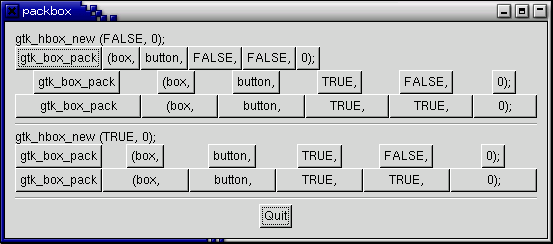
\includegraphics[height=50mm]{images/packbox1.png}
\end{center}
\end{figure}

Ahogy korábban a kódsorokat, most a \textit{widget}sorokat vesszük sorra a minél jobb megértés kedvéért.

\subsubsection{Méretarányos elhelyezés}

\begin{description}
 \item[\textit{expand} = \textit{false}, \textit{fill} = \textit{false}] A konténerben lévő elemek -- ahogy fentiekben fogalmaztunk -- nem akarnak egymás rovására helyet szerezni (\textit{epxand}), így a rendelkezésre álló vízszintes helyet nem is töltik ki, vagyis ezzel a megoldással az egész elemsorra nézve egyfajta balra (\textit{pack\_end} esetén jobbra) zártság alakítható ki.

 \item[\textit{expand} = \textit{true}, \textit{fill} = \textit{false}] Az összkép -- az alatta található sor miatt -- kissé csalóka, mivel az elemek kissé rendezetlennek tűnnek, ugyanakkor arról van szó, hogy minden egyes elem megszerezte magénak -- a saját eredeti méretigényének arányában -- a rendelkezésre álló plusz helyet és az így allokált (\textit{size allocation}) térrészen belül középen helyezkedik el.

 \item[\textit{expand} = \textit{true}, \textit{fill} = \textit{true}] Az egyes elemek nem csak hogy kiterjeszkedtek (\textit{expand}) a korábban fel nem használt területre, de ki is töltik (\textit{fill}) azt, azaz annak terjedelmében rajzolják meg magukat.
\end{description}

Ahogy az az ábrából -- és talán a magyarázatból is -- kitűnik az \textit{fill} opció állításának semmi teteje anélkül, hogy az \textit{expand} be ne lenne kapcsolva, hisz e nélkül nincs semmilyen plusz terült, amire a \textit{widget} magát megnagyobbítva rajzolhatná.

\subsubsection{Homogén elhelyezés}
\index{\textit{homogeneous}}
\index{\textit{fill}}
\index{\textit{expand}}

\begin{description}
 \item[\textit{expand} = \textit{true}, \textit{fill} = \textit{false}] A konténerben lévő elemek -- a már használt kifejezéssel élve -- nem akarnak egymás rovására helyet szerezni (\textit{epxand}), így a rendelkezésre álló vízszintes helyet nem is töltik ki, vagyis ezzel a megoldással az egész elemsorra nézve egyfajta balra (\textit{pack\_end} esetén jobbra) zártság alakítható ki.

 \item[\textit{expand} = \textit{true}, \textit{fill} = \textit{true}] Az összkép -- az alatta található sor miatt -- kissé csalóka, mivel az elemek kissé rendezetlennek tűnnek, ugyanakkor arról van szó, hogy minden egyes elem megszerezte magénak -- a saját eredeti méretigényének arányában -- a rendelkezésre álló plusz helyet és az így allokált (\textit{size allocation}) térrészen belül középen helyezkedik el.
\end{description}

\subsection{Térköz}
\index{\textit{spacing}}
\index{\textit{padding}}

Térköz megadására két lehetőség is kínálkozik a ha elemeket szeretnénk elhelyezni egy \textit{box}ban. Az egyik, hogy magának a konténernek állítunk be létrehozáskor -- vagy akár később -- \textit{spacing}et, vagy az egyes elemek hozzáadásakor adunk meg \textit{padding}et. Hogy mi a különbség a két eset között az alábbi ábra -- ahol az fenti blokkban az első, míg az alsó blokkban a második esetre látunk példát -- jól illusztrálja.

\vspace{12 pt}
\begin{figure}[H]
\begin{center}
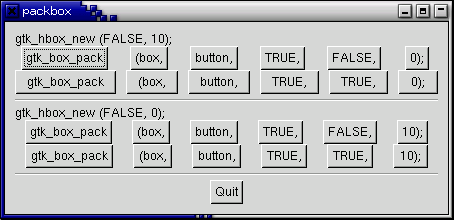
\includegraphics[height=50mm]{images/packbox2.png}
\end{center}
\end{figure}

\subsubsection{Tér az elemek között}
\index{\textit{spacing}}

\begin{description}
 \item[\textit{expand} = \textit{true}, \textit{fill} = \textit{false}] Ez a példa nem mutatja igazán jól meg azt, hogy az elemek között jelenik meg az a térköz, amit a konténer létrehozásakor megadtunk.

 \item[\textit{expand} = \textit{true}, \textit{fill} = \textit{true}] Mivel itt mindkét érték \textit{true}, a \textit{widget}ek a rendelkezésre álló teret teljes egészében kihasználják maguk megrajzolására, eltekintve természetesen a közöttük megjelenő 10 pixel \textit{spacing}től. Érdemes külön megfigyelni a két szélső elemet, azoknak is az ablak széléhez közelebb eső részét a másik megoldással való összehasonlításhoz.
\end{description}

\subsubsection{Tér az elemek körül}
\index{\textit{padding}}

\begin{description}
 \item[\textit{expand} = \textit{true}, \textit{fill} = \textit{false}] A \textit{padding} megadásával a térköz nem az elemek között, hanem azok körül jelenik meg. Ez azt jelenti, hogy minden elem jobb és bal oldalán (\textit{GtkVBox} esetén felül és alul) egyaránt jelentkezik a megadott térköz, ennek okán közöttük annak minimum (függően a \textit{fill} értékétől) a kétszerese.

 \item[\textit{expand} = \textit{true}, \textit{fill} = \textit{true}] Ez az az eset amikor igazán jól látható a \textit{widget}ek között és az azok mellett megjelenő térköz 2:1 aránya. Az előbb -- a szélső widgetek elhelyezkedésénél megfigyelteket -- most hasznosíthatjuk, ha észrevesszük itt a szélső \textit{widget}ek nem tudnak a konténer széléig kiterjeszkedni, lévén két oldalról ki vannak párnázva (\textit{pad}) 10-10 pixellel.
\end{description}

\section{A kód}

A fenti példaprogramok forrása, illetve azok eredetijei, a \textit{FLOSSzine}, valamint a \textit{GTK+} oldalain az alábbi linkeken érhetőek el:
\ \\\\
\url{http://www.flosszine.org/sources/gtk_packbox.c}\\
\url{http://library.gnome.org/devel/gtk-tutorial/2.17/x387.html}

\subsection{Fordítás és linkelés}

A korábbiakhoz hasonlóan az alábbi parancssorok segítségével fordíthatóak elemzett programjaink:

\small
\ \\
\texttt{gcc gtk\_packbox.c -o gtk\_packbox \`{}pkg-config {-}-cflags {-}-libs gtk+-2.0}
\normalsize

\subsection{Futtatás}

Próbáljuk ezúttal a \texttt{./gtk\_packbox 1|2|3}, illetve a \texttt{./gtkmm\_packbox 1|2|3} parancsokkal abban a könyvtárban, ahol a fordítást elkövettük, ahol a paraméter a teszt sorszáma, abban a sorrendben, ahogy azokat itt is ismertettük (a 3. természetesen ráadás).

\subsection{Eredmény}

Ha netán úgy érezzük mégsem világos mi is történik, mikor és miért a konténerekbe pakolás kapcsán ne adjuk fel. Elsőre talán az egész mechanizmus jelentősége sem szembetűnő, ugyanakkor érdemes próbálkozni, azaz venni a forrást és játszani a különböző értékekkel (\textit{fill}, \textit{expand}, \textit{spacing}, \textit{padding}), illetve a létrehozott ablak átméretezésével.

\nocite{gtktut}
\nocite{gtkmmtut}
\nocite{ggad}
\nocite{gtktutmagy}

\addcontentsline{toc}{section}{Hivatkozások}
\bibliography{containers}
\bibliographystyle{plain}

\end{document}

